\documentclass[12pt,a4paper]{article}

\usepackage[utf8]{inputenc} 
\usepackage[spanish]{babel}
\decimalpoint
\setlength{\parskip}{0.5\baselineskip} 
\usepackage{fullpage}
\usepackage[procnames]{listings}
\usepackage{fancyhdr}
\usepackage{lastpage}
\usepackage{xcolor}
\usepackage{booktabs}
\usepackage{graphicx}
\usepackage{subcaption}
\usepackage[fleqn]{amsmath}
\parindent 0in 
\setlength{\mathindent}{0pt}
\usepackage{float}
\usepackage{hyperref}


%% DEFINICIONES
\newcommand{\TODO}[1]{{\huge \color{red} \textbf{TODO: }#1 }}
\newcommand{\todo}[1]{{\large \color{red} \textbf{TODO: }#1 }}
\newcommand{\rev}[1]{{\color{green} #1 }}
\newcommand{\HRule}{\rule{\linewidth}{0.5mm}}
\newcommand{\pong}{\emph{Pong} }

\definecolor{bluekeywords}{rgb}{0,0,1}
\definecolor{greencomments}{rgb}{0,0.5,0}
\definecolor{redstrings}{rgb}{0.64,0.08,0.08}
\definecolor{xmlcomments}{rgb}{0.5,0.5,0.5}
\definecolor{types}{rgb}{0.17,0.57,0.68}


%%%%%%%%%%%%%%%%%%%%%%%%%%%%%%%%%%%%%%%%%%%%%%%%%%%%%%%%%%%%%%%%%%%%%%%%%%%%%%%%
\begin{document} 

\begin{titlepage}

  \begin{center}


    % Upper part of the page
    
\includegraphics[width=0.4\textwidth]{images/escudo.jpg}\\[1cm]    

    \textsc{\LARGE Universidad Complutense de Madrid}\\[1.5cm]

    \textsc{\Large Sistemas Empotrados Distribuidos}\\[0.5cm]


    % Title
    \HRule \\[0.4cm]
           { \huge {\bfseries PONG:}\vspace{0.3cm}\\
             Diseño e implementación sobre\\FPGA y ARM}\\[0.4cm]
           
           \HRule \\[1.5cm]

           \vspace{1.5cm}
           % Author and supervisor
           \hfill\emph{Autores:}\\
           \hfill Luis María Costero Valero\\
           \hfill Jesús Javier Doménech Arellano
           
           \vfill
           
           % Bottom of the page
           {\large Mayo 2016}
           
  \end{center}
  
\end{titlepage}


%
%
%%%
%%% Local Variables:
%%% mode: latex
%%% TeX-master: "../main.tex"
%%% End:

\tableofcontents
\listoffigures

\clearpage{}
\section{Introducción}
\label{s1:sec:Introduccion}

\subsection{El juego}
\label{s1:subsec:elJuego}
El videojuego \pong es uno de los videojuegos más conocidos por todos,
publicado por Atari en 1972. \pong consiste en un juego para dos personas,
en el que el objetivo es hacer rebotar a una pelota para que el oponente no
pueda golpearla y pierda.
\begin{figure}[h]
  \centering
  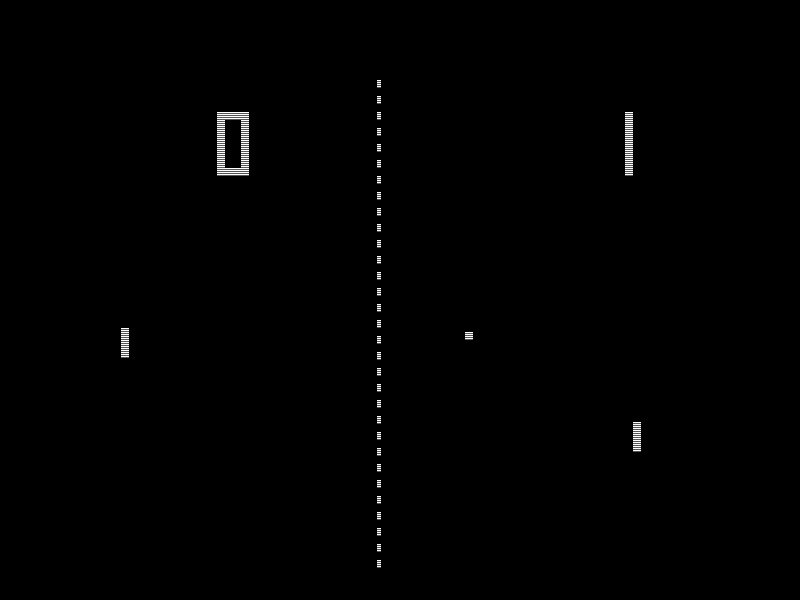
\includegraphics[width=0.4\textwidth]{images/pong.png}
  \caption{Imagen del juego original.}
  \label{s1:fig:pong}
\end{figure}

Para controlar la pelota, cada jugador dispone de una raqueta situada en
uno de los extremos de la pantalla, la cual únicamente pude desplazarse en
vertical. Cuando la pelota golpea una de estas raquetas, ésta cambia el
sentido horizontal de movimiento, dirigiéndose al otro jugador. Según en
que parte de la raqueta golpee la bola, ésta también modifica su componente
de movimiento vertical. De igual manera, cuando la pelota golpea el borde
superior o inferior del juego, también ve modificado su movimiento.  Se
considera que un jugador pierde cuando no es capaz de golpear la pelota y
ésta sale del juego por su lado de la pantalla.


\subsection{Descripción del proyecto}
\label{s1:subsec:objetivos}
El trabajo realizado consiste en el diseño e implementación del juego \pong
sobre una arquitectura distribuida formada por una FPGA Spartan~3~\cite{Spartan3}, y
dos maletines ARM S3C44B0X~\cite{maletinARM}, comunicados entre ellos
mediante UARTs.

La FPGA es el componente encargado de la lógica del juego. En él se
realizan todos los cálculos de posiciones y choques de la pelota. También
se lleva control de las puntuaciones. Además, sobre la FPGA se han
implementado dos módulos adicionales, uno encargado de la comunicación con
los maletines mediante UARTs, y otro para mostrar el juego en un monitor
VGA.\\
Los maletines ARM son utilizados para leer los movimientos de los jugadores
(mediante pulsadores y teclado matricial) y comunicárselo a la FPGA
mediante una UART. Además, por motivos de diseño de la FPGA (sólo posee un
puerto UART), los maletines están diseñados para ser conectados en serie y
retransmitir los mensajes de un maletín al siguiente, hasta llegar a la
FPGA. La puntuación del juego también es mostrada por los \textit{display}
8-segmentos de la placa.

En la figura figura~\ref{s1:fig:vista_general_sistema} se puede ver una
descripción general del sistema.\\

\begin{figure}[h]
  \centering
  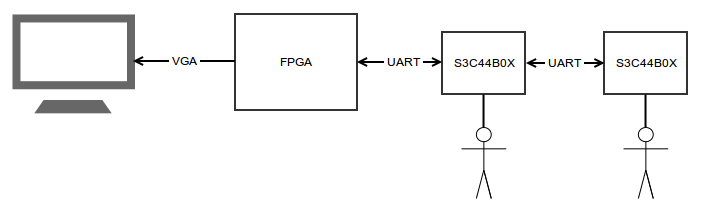
\includegraphics[width=0.8\textwidth]{images/descripcion_general.png}
  \caption{Descripción general del sistema.}
  \label{s1:fig:vista_general_sistema}
\end{figure}


La memoria está organizada de la siguiente forma:
en la sección~\ref{s2:sec:Disenyo} se muestra el modelado realizado por el
sistema, y diversos diagramas que describen el comportamiento del mismo. La
sección~\ref{s3:sec:Implementacion} muestra los aspectos más relevantes en
la implementación. Y para finalizar, la sección~\ref{s4:sec:Conclusiones}
muestra unas conclusiones y trabajo futuro a realizar si se desea seguir
con el proyecto.








%
%
%%%
%%% Local Variables:
%%% mode: latex
%%% TeX-master: "../main.tex"
%%% End:



\clearpage{}
\section{Diseño}
\label{s2:sec:Disenyo}

\subsection{Componentes del sistema}
\label{s2:subsec:sistema-entero}
A la hora de realizar el sistema, se ha decidido utilizar los siguientes
componentes:
\begin{itemize}
\item \emph{FGPA}, que como se ha comentado en la sección anterior, es la
  encargada de realizar los cálculos del juego, interpretar las órdenes de
  los usuarios, y mostrar el juego mediante un monitor VGA.
\item \emph{Maletines ARM}, encargados de leer las órdenes de los
  jugadores (mediante pulsaciones en el teclado matricial o los botones de
  la placa) y transmitirlas a la FPGA mediante una UART. Como la FPGA
  utilizada únicamente posee una UART, los maletines se pueden conectar en
  serie, y transmitir los mensajes de uno hacia el siguiente hasta que
  lleguen a la FPGA (ver sección~\ref{s3:subsec:maletines}). Además, la
  FPGA transmite la información de puntuación a los maletines, los cuales
  la muestran mediante sus \emph{Display 8-Segmentos}.
\item \emph{Display 8-Segmentos}, utilizado para mostrar la información de
  puntuación.
\item \emph{Pulsadores y teclado matricial}, para que los jugadores
  indiquen sus órdenes de movimiento al sistema.
\item \emph{Monitor VGA}, utilizado para mostrar el juego.
\end{itemize}

A continuación se muestra tanto el comportamiento global del sistema, como
la comunicación entre los distintos componentes. En la sección siguiente
se muestra con más detalle el funcionamiento del componente FPGA
(apartado~\ref{s3:subsec:fpga}) y de los maletines ARM
(apartado~\ref{s3:subsec:maletines}).

\subsection{Comportamiento del sistema}
\label{s2:subsec:comportamiento}
El núcleo del sistema es la FPGA que lleva todo el control del juego y
los maletines ARM actúan de periféricos. 

Entonces el comportamiento del sistema (resumido en la
figura~\ref{s2:fig:comportamiento}) consiste en un búcle principal,
siguiendo el ciclo del reloj de juego,
donde se va calculando la situación del juego y este recibe
modificaciones externas de manera distribuída que modifican los
biestables que componen el escenario, en este caso la posición de las
raquetas de cada jugador.  

Por otro lado, la FPGA notifica a los maletines el estado del juego en
cuanto a puntuaciones. Esta forma de abstraer el control de los
jugadores de la lógica del juego nos permitiría por ejemplo sustituir
el control por un PS2, como ya hemos indicado, e incluso realizar la
comunicación por medio de un \todo{puerto red} por donde se recibe las
indicaciones de movimiento y se manda la situación del juego. 

Otro búcle del sistema es el de pintado VGA explicado en la
sección~\ref{TTTT}.\todo{Seccion para la VGA!!}

En los maletines ARM el sistema es mucho más sencillo (explicado en
detalle en la sección~\ref{s3:subsec:maletines}) ambos actúan de igual
manera. Los maletines creen ser el más cercano a la FPGA y actúan como
jugador 1, pero el maletin más cercano convierte al jugador 1 en
jugador 2. Este método permite conectar en serie cualquier cantidad de
maletines y tendríamos un juego de N jugadores si fuese
necesario\footnote{En la última sección~\ref{s4:sec:Conclusiones}
  pueden verse detalles de como podría convertirse en un juego de
  cuatro jugadores}, desde el punto de vista de la FPGA se trata de un único
maletín o teclado en el que juegan todos los jugadores de manera simultánea. \\

Este sistema podría mostrar la debilidad de un posible retardo en las
acciones realizadas por el jugador del maletín más lejano pero esto se
compensa tal y como se exlica en la sección~\ref{s3:subsubsec:clocking} al llevar
diferentes relojes en cada parte del sistema, la recepción de comandos
es mucho más rápida que el reloj de movimiento del juego así que por
mucho que llegase un poco más tarde llegaría antes del siguiente ciclo
de reloj de movimiento.

\begin{figure}[h]
  \centering
  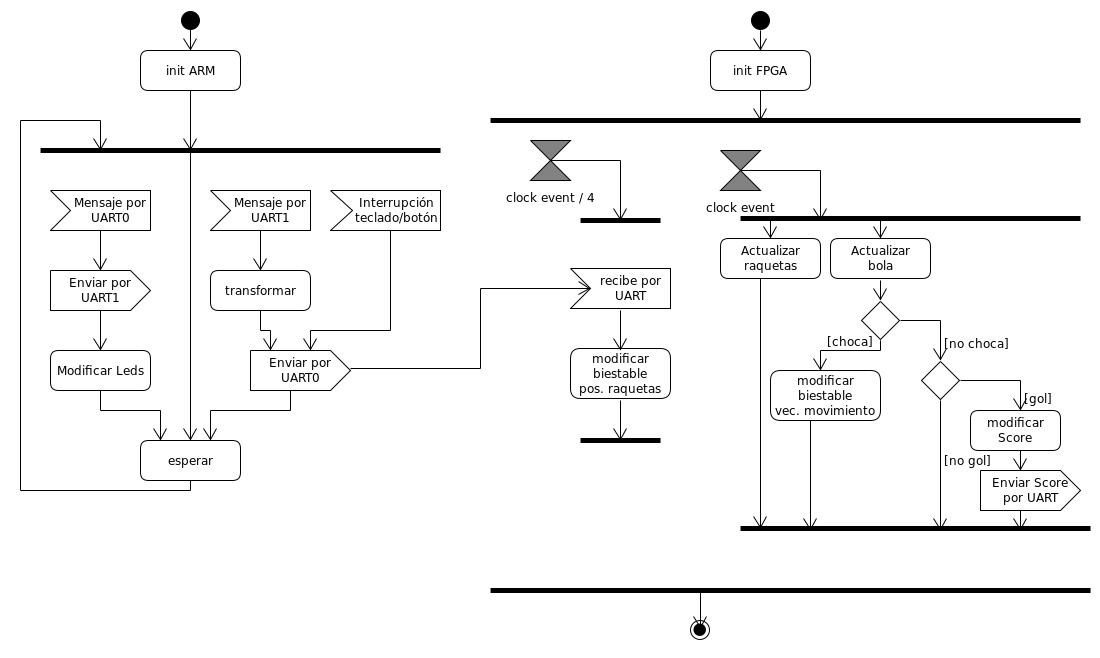
\includegraphics[width=1.0\textwidth]{images/sistema.png}
  \caption{Diagrama de Actividad del sistema (sin VGA).}
  \label{s2:fig:comportamiento}
\end{figure}

\subsection{Comunicación entre componentes}
\label{s2:subsec:comunicacion}
\rev{Como se ha mencionado anteriormente, el sistema está controlado por
  una FPGA, la cual ejecuta varios bucles de manera paralela para modificar
  el estado del juego y pintar en el monitor VGA los elementos del
  juego}. El resto de componentes (maletín, display 8-Segmentos,
pulsadores, $\ldots$) sirven para modificar el estado del juego mediante
comunicaciones con la FPGA, que permiten que esta calcule las nuevas
posiciones. Según qué componentes interactúen entre ellos, la comunicación
usada es diferente:
\begin{itemize}
\item \emph{FPGA -- VGA:} Comunicación unidireccional utilizando el
  conector VGA. Se utilizan 9 líneas para los colores (3 para cada color),
  y 2 líneas adicionales para la sincronización horizontal y vertical
  respectivamente. \rev{Si da tiempo, el diagrama ?? muestra la máquina de
    estados que controla el dibujado en pantalla.} (Más información se
  puede encontrar en~\cite{Spartan3-StarterKit}).
\item \emph{Pulsadores -- Maletín:} Detección de pulsaciones mediante
  interrupciones en la placa.
\item \emph{Maletín -- Maletín:} Comunicación mediante UARTs. El diseño
  utilizado permite conectar varios maletines en serie, por lo que el
  comportamiento general de los maletines es recibir la información por una
  UART, procesarla y reenviarla por la otra UART. Si la información es
  recibida por la \rev{UART0}, se trata de otro maletín que envía
  información a la FPGA, mientras que si se recibe por la \rev{UART1},
  es la FPGA la que envía información a los maletines.
\item \emph{FPGA - Maletín:} Comunicación mediante UART. Como la FPGA
  únicamente dispone de un puerto UART, la conexión de los maletines se
  hace en serie, siendo los maletines intermedios encargados de reenviar la
  información en ambos sentidos (hacia la FPGA o hacia el resto de
  maletines).
\end{itemize}

La figura~\ref{s2:fig:secuencia} muestra de manera resumida la comunicación
entre los distintos componentes. Como se puede observar, la FPGA posee dos
grandes bucles\footnote{Más información sobre los bucles de la FPGA, y de
  manera especial sobre los distintos relojes utilizados, se puede encontrar
en~\ref{s3:subsubsec:clocking}.} encargados de calcular el estado del juego, y de pintar en
el monitor. Cuando un jugador pulsa un botón, la información es transmitida
a la FPGA a través de los maletines, modificando el cálculo del estado del
juego. En el caso de que un jugador falle, la FPGA envía información hacia
los maletines para informar de la nueva puntuación.

\begin{figure}[h]
  \centering
  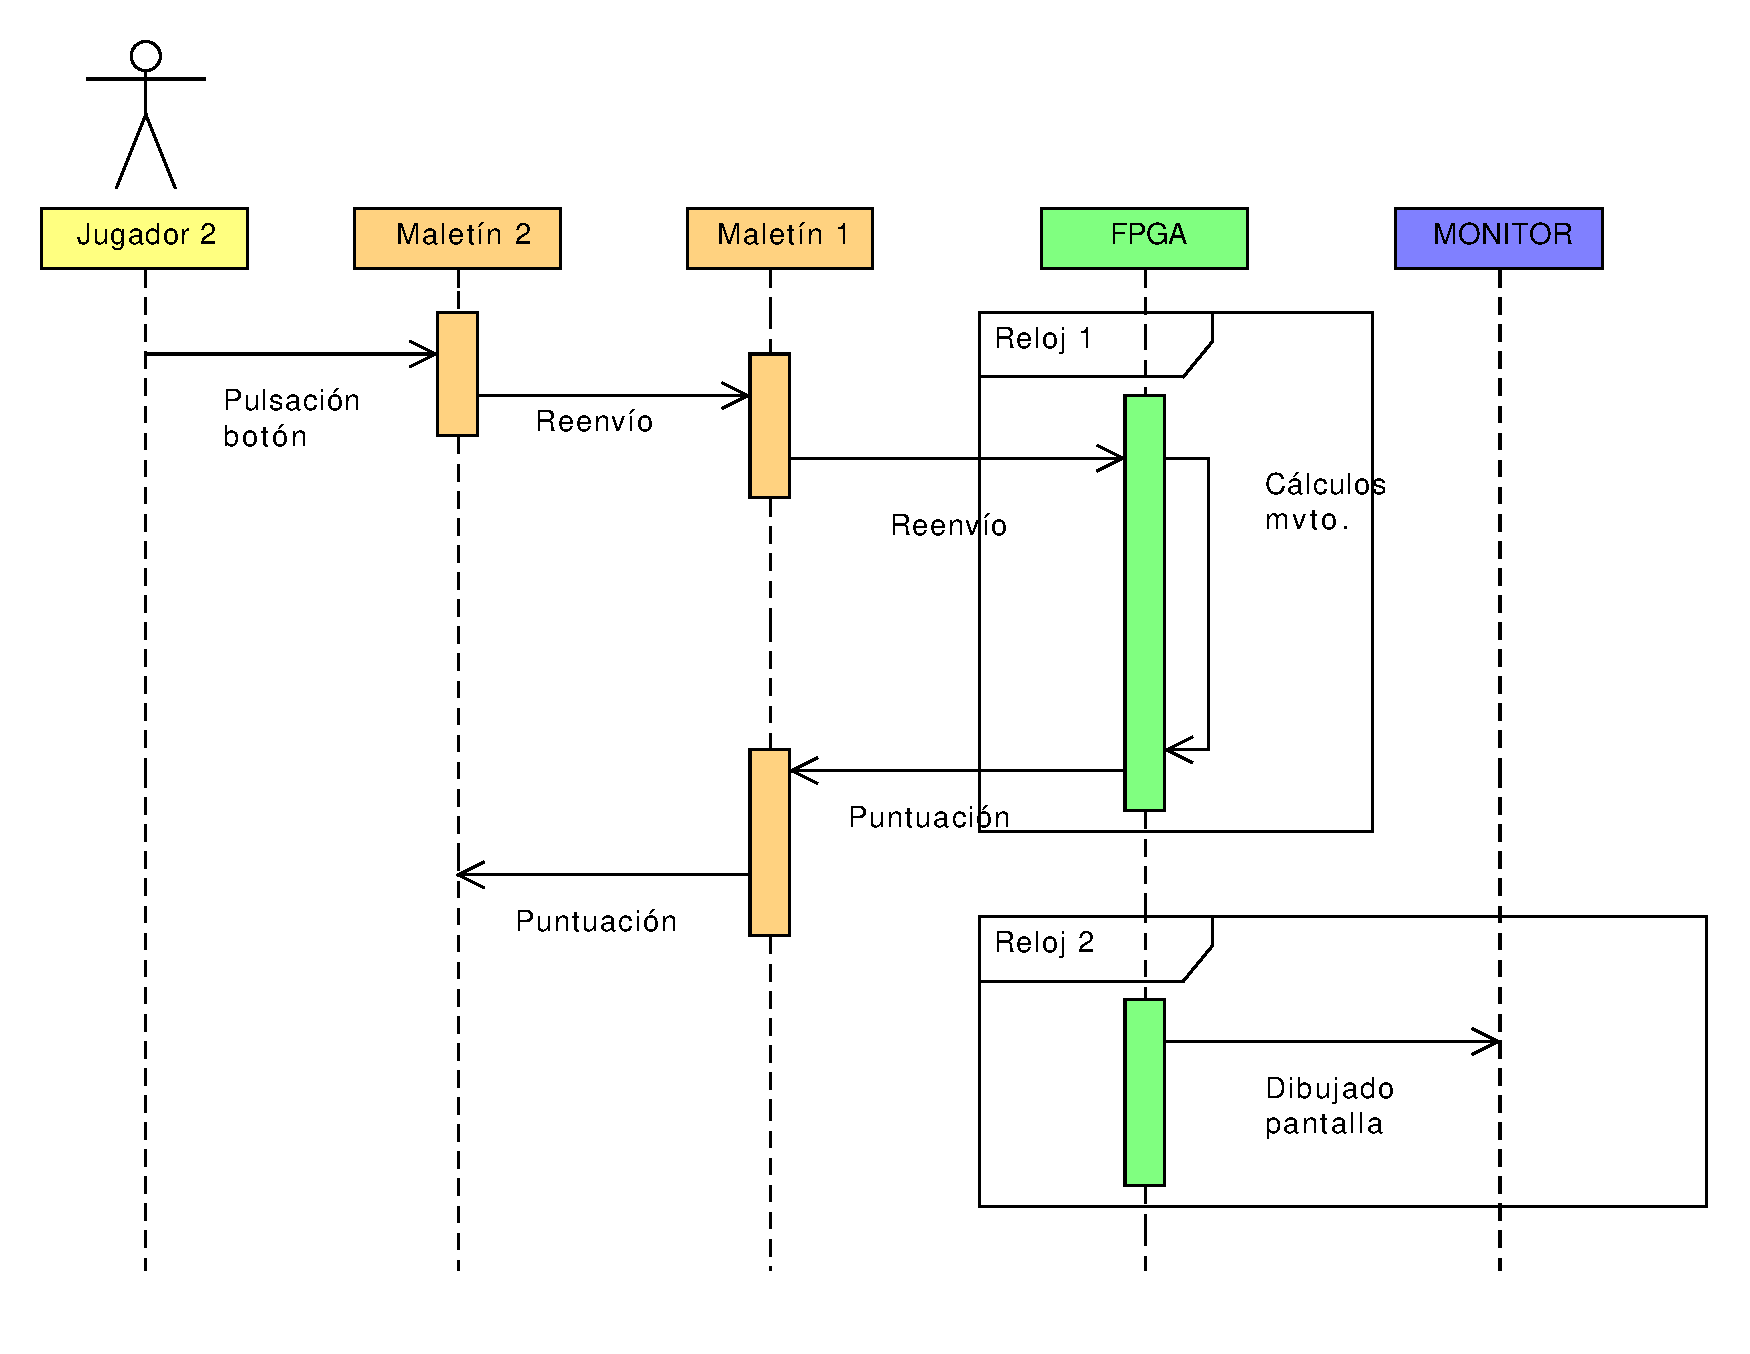
\includegraphics[width=1.0\textwidth]{images/secuencia.pdf}
  \caption{Diagrama de secuencia entre los distintos componentes.}
  \label{s2:fig:secuencia}
p\end{figure}



%
%
%%%
%%% Local Variables:
%%% mode: latex
%%% TeX-master: "../main.tex"
%%% End:



\clearpage{}
\section{Implementación}
\label{s3:sec:Implementacion}


\subsection{FPGA}
\label{s3:subsec:fpga}
Para la implementación del juego sobre la FPGA, se ha decidido implementar
distintos módulos, conectados entre ellos, que permiten calcular el estado
del juego. La relación entre los distintos módulos se puede ver en la
figura~\ref{s3:fig:componentes-fpga-a}. Además, para que el juego pueda
funcionar a una velocidad adecuada, pero se pueda comunicar con los
maletines, y además pintar en el monitor VGA, cada módulo está controlado
por su propio reloj, como se explica en la sección~\ref{s3:subsubsec:clocking}.
y se muestra en la figura~\ref{s3:fig:componentes-fpga-clocking}. 


\begin{figure}[h]
  \centering
  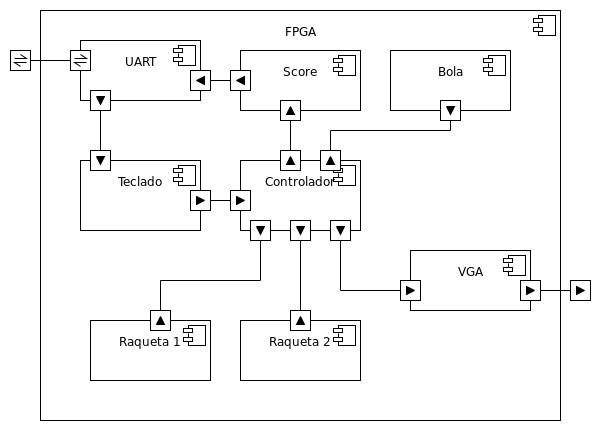
\includegraphics[width=1.0\textwidth]{images/fpga_componentes_v2.png}
\caption{Diagrama de componentes implementados en la FPGA. }
\label{s3:fig:componentes-fpga-a}
\end{figure}

Como se muestra en la figura, los módulos de los que está compuesta la
implementación sobre la FPGA son:
\begin{itemize}
\item \emph{Módulo UART:} módulo encargado de leer y enviar información a
  través de la UART de la FPGA. Posee señales de control para indicar
  cuándo un dato se ha recibido, o cuando está ocupada enviando
  información.
\item \emph{Módulo teclado:} traduce la información recibida por la UART a
  comandos internos entendidos por el juego. Este diseño nos permite
  desacoplar el módulo teclado de la UART y cambiarlo por otros módulos
  que interpreten otros dispositivos de entrada, como puede ser un teclado
  PS2.
\item \emph{Módulo raquetas:} contienen la información de la posición de
  las raquetas. Las teclas leídas del módulo teclado modifican la posición
  de este módulo. Este módulo se encuentra instanciado varias veces, una
  por cada raqueta del juego.
\item \emph{Módulo bola:} calcula en cada pulso del reloj del juego la
  nueva posición de la pelota. Además, recibe la información de las palas
  para calcular los rebotes con ellas, o si un jugador gana el partido
  actual. Si es el caso, el módulo informa al módulo controlador para que
  anote e informe del cambio de puntuación.
\item \emph{Módulo puntuación:} encargado de guardar la información de los
  partidos. Cuando un jugador consigue un tanto, se comunica con el módulo
  de la UART para enviar la información a los maletines.
\item \emph{Módulo VGA:} a partir de la información del módulo bola y de
  los módulos de raquetas, dibuja en un monitor VGA el juego.
\item \emph{Módulo controlador:} encargado de llevar la máquina de estados
  principal del juego y comunicar los diferentes módulos entre sí.
\end{itemize}

\subsubsection{Gestión de los relojes}
\label{s3:subsubsec:clocking}
Aunque el diseño y ejecución del juego sobre la FPGA tiene muchas ventajas
(la mayoría relativas a la facilidad de realizar cálculos en paralelo), es
necesario sincronizar cada uno de los módulos entre ellos. Además, el
diseño elegido para la implementación hace que cada módulo utilice un reloj
distinto. Los distintos relojes utilizados se muestran en la
figura~\ref{s3:fig:componentes-fpga-clocking}, donde cada color refleja el
reloj utilizado en los módulos que se indican.

\begin{figure}[h]
  \centering
  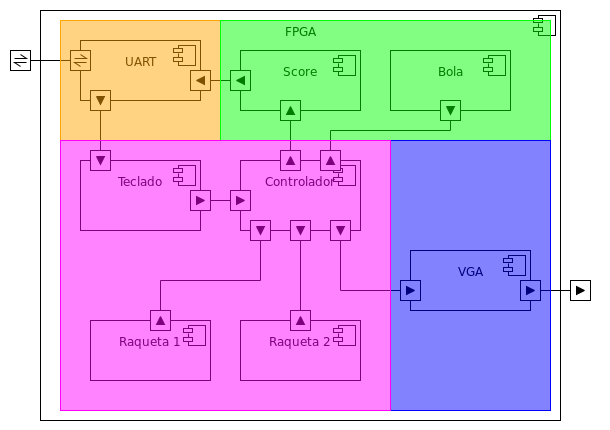
\includegraphics[width=0.8\textwidth]{images/fpga_componentes_timing_v2.png}
  \caption{Distintos relojes utilizados.}
  \label{s3:fig:componentes-fpga-clocking}
\end{figure}


Más concretamente se ha decidido utilizar cuatro relojes sobre la FPGA,
cada uno con un propósito distinto:
\begin{itemize}
\item \emph{Reloj principal (rosa):} reloj principal de la
  placa. Proporciona un pulso cada 100 ns. Es utilizado para leer los datos
  procesados en tiempo real por la UART e informar a las raquetas de su
  nueva posición. Se ha decidido utilizar un reloj rápido ya que se
  consigue reaccionar de manera más rápida a las pulsaciones del
  jugador. Para no perder datos con el módulo de la UART (al tener
  distintos relojes), la información es almacenada en un biestable hasta
  que ésta es leída.
\item \emph{Reloj UART (naranja):} se trata del mismo reloj utilizado para
  la transmisión con la UART en los maletines ARM.
\item \emph{Reloj de juego (verde):} utilizado para calcular los
  movimientos de la pelota. Se trata de una división del reloj principal
  del juego, que al ser más lento permite visualizar los movimientos por la
  pantalla y hacer que el jugador sea consciente de lo que ocurre y le dé
  tiempo a reaccionar.
\item \emph{Reloj VGA (azul):} necesario para transmitir por el
  protocolo VGA. Según este protocolo, el reloj debe ir a 25MHz (un cuarto
  del reloj principal del juego).
\end{itemize}

\subsection{Maletines ARM}
\label{s3:subsec:maletines}
% \todo{Escribir esto, haciendo referencia a~\ref{s3:fig:FSM_maletin}. Si se
%   decide mover la imagen a~\ref{s2:subsec:sistema-entero}, inventarse que
%   poner. }\\
% \todo{Sería interesante explicar lo del tecldo, y lo que se  hace para
%   poder conectar varios maletines en serie.}

Como se ha dicho anteriormente, la FPGA utilizada solamente posee una
conexión UART, por lo que el diseño elegido para los maletines es
conectarlos en serie. Además, todos los maletines ejecutan el mismo código,
encargado de transmitir la información de una UART hacia la otra. La
figura~\ref{s3:fig:FSM_maletin} muestra el comportamiento de los maletines.

% Todos los maletines ejecutan el mismo código, como ya se ha dicho
% anteriormente van conectados en serie mandando comandos de maletín a
% la FPGA y recibiendo las puntuaciones de la FPGA a los maletines. \\

% El funcionamiento de los maletines ARM se puede apreciar en la
% figura~\ref{s3:fig:FSM_maletin}. La primera fase es configurar las
% interrupciones de los botones y el teclado matricial, se inicializan
% los display 8 segmentos y se configuran las UARTs. \\


\begin{figure}[h]
  \centering
  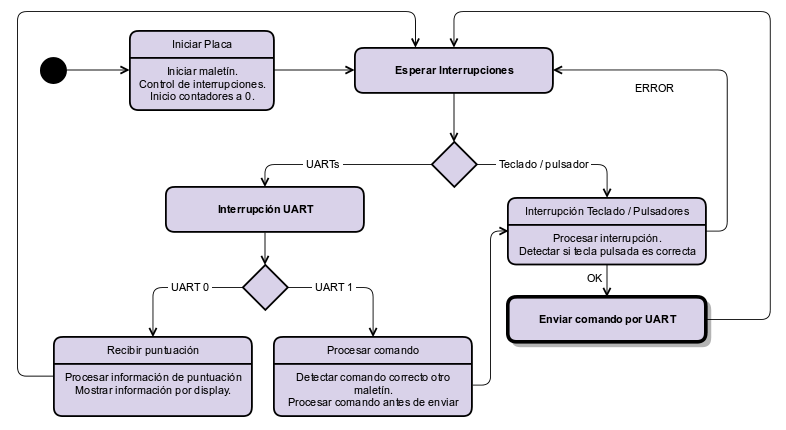
\includegraphics[width=0.8\textwidth]{images/maletin_fsm.png}
  \caption{FSM describiendo el comportamiento de los maletines.}
  \label{s3:fig:FSM_maletin}
\end{figure}


Al iniciar las placas, lo primero ejecutado es la inicialización de la
misma, las conexiones UARTs, activación de interrupciones y marcar los
contadores de puntuación a 0. A continuación se entra en un bucle que va a
controlar el juego. Si se recibe una interrupción de un pulsador o del
teclado matricial, esta pulsación se procesa y se envía por la UART1 al
siguiente elemento de la cadena (que puede ser otro maletín o la FPGA). Si
se detecta la interrupción asociada a un puerto UART, pueden distinguirse
dos casos:
\begin{itemize}
\item Interrupción en UART0. Indica que la información recibida proviene de
  otro maletín. En este caso, se procesa la información para indicar que no
  la ha generado el maletín, y se envía por la UART1 al siguiente elemento
  de la cadena (que va a ser la FPGA en el caso de tener únicamente dos
  maletines).
\item Interrupción en UART1. Indica que la información recibida proviene o
  bien de la FPGA, o bien la está retransmitiendo el otro maletín. La
  información es procesada (información relativa a la puntuación), y
  mostrada por los display 8-Segmentos.
\end{itemize}




%
%
%%%
%%% Local Variables:
%%% mode: latex
%%% TeX-master: "../main.tex"
%%% End:



\clearpage{}
\section{Conclusiones}
\label{s4:sec:Conclusiones}

\begin{itemize}
\item Conclusiones
\item Cosas a mejorar
\item Trabajo futuro
\end{itemize}







%
%
%%%
%%% Local Variables:
%%% mode: latex
%%% TeX-master: "../main.tex"
%%% End:





\clearpage{}
\bibliographystyle{ieeetr}
\bibliography{references} 


\end{document}



%
%
%%%
%%% Local Variables:
%%% mode: latex
%%% TeX-master: "./main.tex"
%%% End:

